%%%%% Document Setup %%%%%%%%

\documentclass[12pt, onecolumn]{revtex4}    % Font size (12pt) and column number (one or two).

\usepackage[a4paper, left=2.5cm, right=2.5cm, top=2.5cm, bottom=2.5cm]{geometry}  % Defines paper size and margin length

\renewcommand{\baselinestretch}{1}     % Defines the line spacing

\usepackage{subcaption}

\usepackage[font=small, labelfont=bf]{caption}                      % Defines caption font size and caption title bolded
\captionsetup[figure]{justification=justified, singlelinecheck=off, font=footnotesize} 
\captionsetup{compatibility=false}

\usepackage{graphics,graphicx,epsfig,ulem}	% Makes sure all graphics works
\usepackage{amsmath} 						% Adds mathematical features for equations

\usepackage{etoolbox}                       % Customise date to preferred format
\makeatletter
\patchcmd{\frontmatter@RRAP@format}{(}{}{}{}
\patchcmd{\frontmatter@RRAP@format}{)}{}{}{}
\renewcommand\Dated@name{}
\makeatother

\usepackage{fancyhdr}

\pagestyle{fancy}                           % Insert header
\renewcommand{\headrulewidth}{0pt}
%\lhead{\small Jacky Cao}                        
\rhead{\small }                

\def\thesection{\arabic{section}}
\def\thesubsection{\alph{subsection}}

\def\bibsection{\section*{References}}        % Position reference section correctly
\setcitestyle{authoryear,round}
\setlength\bibhang{0.2in}
\usepackage[colorlinks]{hyperref}
\hypersetup{
    colorlinks=true,
    linkcolor=black,
    citecolor=black,    
    urlcolor=black,
}

\usepackage{tabularx}

%%%%% Document %%%%%
\begin{document}                     

\title{Prediction limitations with ENSO models and the spring predictability barrier} 
%\date{Submitted: \today{}} \author{Jacky Cao}

\maketitle
\thispagestyle{plain} % produces page number for front 

\section{Introduction}
% Introducing ENSOs and what EN and SO are individually and then setting the problem from the offset 
The El Ni\~{n}o Southern Oscillations (ENSOs) are generally known as a composite weather phenomena originating in the Pacific Ocean producing lasting teleconnections on the global climate system. The El Ni\~{n}o component of ENSO can be approximately considered to be an oceanic warming event which disrupts the normal Pacific circulation at irregular intervals of 2--7 years, whilst the Southern Oscillations are an inter-annual flip of the tropical sea level pressure between the western and eastern Pacific leading to the weakening and strengthening of the easterly trade winds across the ocean. To produce a conclusive theory for ENSOs one must be able to describe and understand the complete underlying mechanisms. One such hypothesis has yet to arise, however various attempts have been made to comprehend individual components and effects. \\
% words: 127

% How Bjerknes, Zebiak and Cane set the stage for ENSO research 
\cite{doi:10.1175/1520-04931969097} first theorised that a positive ocean-atmosphere feedback system would result in an El Ni\~{n}o event. An initial positive sea surface temperature (SST) anomaly in the eastern Pacific would reduce the east-west SST gradient which leads to the strengthening of the Walker circulation and thus the production of weaker trade winds across the equatorial Pacific. In a complete ENSO theory this positive system would be counterbalanced by a negative loop which returns the Pacific to its ``normal'' (pre-ENSO) state. Whilst Bjerknes' hypothesis fails to provide a negative feedback mechanism, \cite{Zebiak:1987aa} presented a model which demonstrated and outlined the coupling between the atmosphere and the ocean to produce an ENSO event. The atmospheric component used was a linear Gill-type model \citep{Gill:1980aa} which describes the atmosphere's response to SST anomalies, and the ocean represented by a low-gravity system which is forced by the wind stress from the atmospheric constituent. \\
% words: 147

With their model they were able to replicate features observed during ENSO events such as equatorial westerly wind anomalies in the central Pacific and large SST anomalies in the eastern Pacific, on top of that they were able to predict the onset of the 1986--1987 and 1991--1992 ENSO events. Despite this success, they recognised their limited ability in simulating the real complete system as detailed comparisons with observational data would reveal discrepancies in their atmospheric and oceanic simulations. Furthermore, the short warm episodes in 1993 and 1994 would be missed in the predictions made with the Zebiak-Cane (ZC) model. This therefore requires more sophisticated models to better describe and forecast ENSO events.
% words: 112

\section{Prediction limitations and the Zebiak-Cane Model}

The prediction of ENSO events is particularly difficult as there are generally two types of El Ni\~{n}o events to account for. The first are canonical events which generally develop along the South American coast and then propagate westwards across the Pacific, ``Eastern-Pacific'' events \citep{rasmusson1982variations}. The second type of events have non-propagating warm SST concentrated mostly in the central Pacific, ``Central-Pacific'' events \citep{ashok2007nino}. In an attempt to test whether the ZC model can predict either types of events, it was demonstrated by \cite{duan2013behaviors} that the model tended to do well whilst simulating Eastern-Pacific (EP) events and functioned badly when reproducing Central-Pacific (CP) events. This indicates that the ZC model may just contain the physics to explain EP events and that alterations would be required to additionally account for other events. \\
% words: 129

Additional challenges for ENSO forecasting arise due to the nonlinear and complex coupling between the ocean and atmospheric systems. Within the ZC model this relationship was constrained as a result of the researchers' initial assumptions and parameter choices when constructing their theory. For example with the simulation of monthly mean SST anomalies in the atmosphere model, concessions had to be made to ensure accurate results could be produced whilst the analysis not being computationally costly. Further experimentation would exhibit that the amplitude and time scale of the ENSO cycles would be sensitive to changes within the coupled mathematical model: an increase (or decrease) in the strength of the coupling between the atmosphere and ocean would lead to increase (or decrease) in the amplitudes and periods. \\
% words: 125

It is therefore evident that the ZC model is a simplification of the real climate system and improvements must be made to provide a better fit with the observational data. Theoretical modifications of the individual atmospheric and oceanic components plus of their inter-relationship would be key in developing the theory further. Several modern ENSO oscillator theories (Table \ref{table:enso_oscillators}) employ the ZC model as a basic foundation whilst making adjustments to parts of the mathematical modelling thus improving their ability to explain and account for various ENSO effects.
% words: 87

\begin{table}[htbp]
\renewcommand{\arraystretch}{1.0}
%\begin{tabular}{c@{\hskip 20pt}c} 
\begin{tabular}{|p{7cm}|p{9cm}|}
 \hline
 \textbf{Theory} & \textbf{Main component(s)} \\ [0.5ex] 
 \hline
 The Delayed Oscillator \citep{Suarez:1988aa, Battisti:1988aa} & Considers the effects of equatorially trapped oceanic wave propagation. \\
 \hline
 The Recharge Oscillator \citep{Jin:1997aa} & Considers the buildup of warm water in the western Pacific as a precondition to the development of El Ni\~{n}o. \\
 \hline
 The Western Pacific Oscillator \citep{Weisberg:1997aa, wang1999effects} & Considers the role of the western Pacific and off-equatorial SST SST anomalies in the western Pacific. \\
 \hline
 The Advective-Reflective Oscillator \citep{Picaut663} & Considers the importance of the positive feedback of zonal currents that advect the western Pacific warm pool towards the east during El Ni\~{n}o.  \\
 \hline
 The Unified Oscillator \citep{wang2001unified} & Considers dynamics and thermodynamics of a coupled ocean-atmosphere system which is similar to Zebiak-Cane. \\
 \hline
\end{tabular}
\captionof{table}[ENSO Oscillators]{Various ENSO oscillator theories and their main differences from the ZC model.}
\label{table:enso_oscillators}
\end{table}

Changes to the ZC model are not limited to just the atmospheric and oceanic components, as a response to the model failing to agree with observations from 1992 to 1995, \cite{qian1997multiple} introduced planetary scale Hadley and Walker cells which improved the prediction of equatorial eastern Pacific SST anomalies for 1970--1971 and in 1992--1995. \\
% words: 53

However further shortfalls exist within the modelling for ENSOs which limits their accuracy and applicability. In particular, there is a limitation found in many models known as the ``spring predictability barrier'' where the seasonal predictions for ENSOs made during or before boreal spring (March--May) have much lower skill than those made at other times of the year \citep{torrence1998annual}. This barrier can be evidenced in oceanic circulation models \citep{latif1992much}, in dynamical-statistical models \citep{balmaseda1994enso}, and in coupled ocean-atmosphere models \citep{goswami1991predictability, xue1994prediction}. To better predict ENSO events, this barrier therefore must be understood and accounted for within climate modelling.
% words: 96

\section{Evidence for the spring predictability barrier}

Examinations of the autocorrelation, persistence, and phase locking of ENSO data sets provides the tools to help discern the predictability barrier. \\
% words: 21

Autocorrelation is the correlation of a data set with a version of it self which has been shifted in time by a certain lag. \cite{trenberth1976spatial} analysed monthly sea level pressures across the Pacific Ocean to conclude that SST and Southern Oscillation Index (SOI) both have high degrees of autocorrelations which agree with observations that ENSO events normally persists for several months. This then allows for a forecast of persistence across several months where the prediction hinges on the starting month of the initial persistence forecast. \\
% words: 85

Persistence is an another analysis of the correlation, however it looks at the fixed-phase correlation between different months within a single time series \citep{troup1965southern}. Contrasting with autocorrelation, which is independent of the starting month, persistence allows you to see any seasonal changes in the correlation between one month and the next. Analysis by \cite{torrence1998annual} of the NINO3 SST and SOI data shows that persistence has distinct structure which is phase locked to an annual cycle. Regardless of starting month, the persistence shows that there is a rapid decline in the March--April--May period (Fig. \ref{fig:persistence_sst_soi}). \\

\begin{figure}
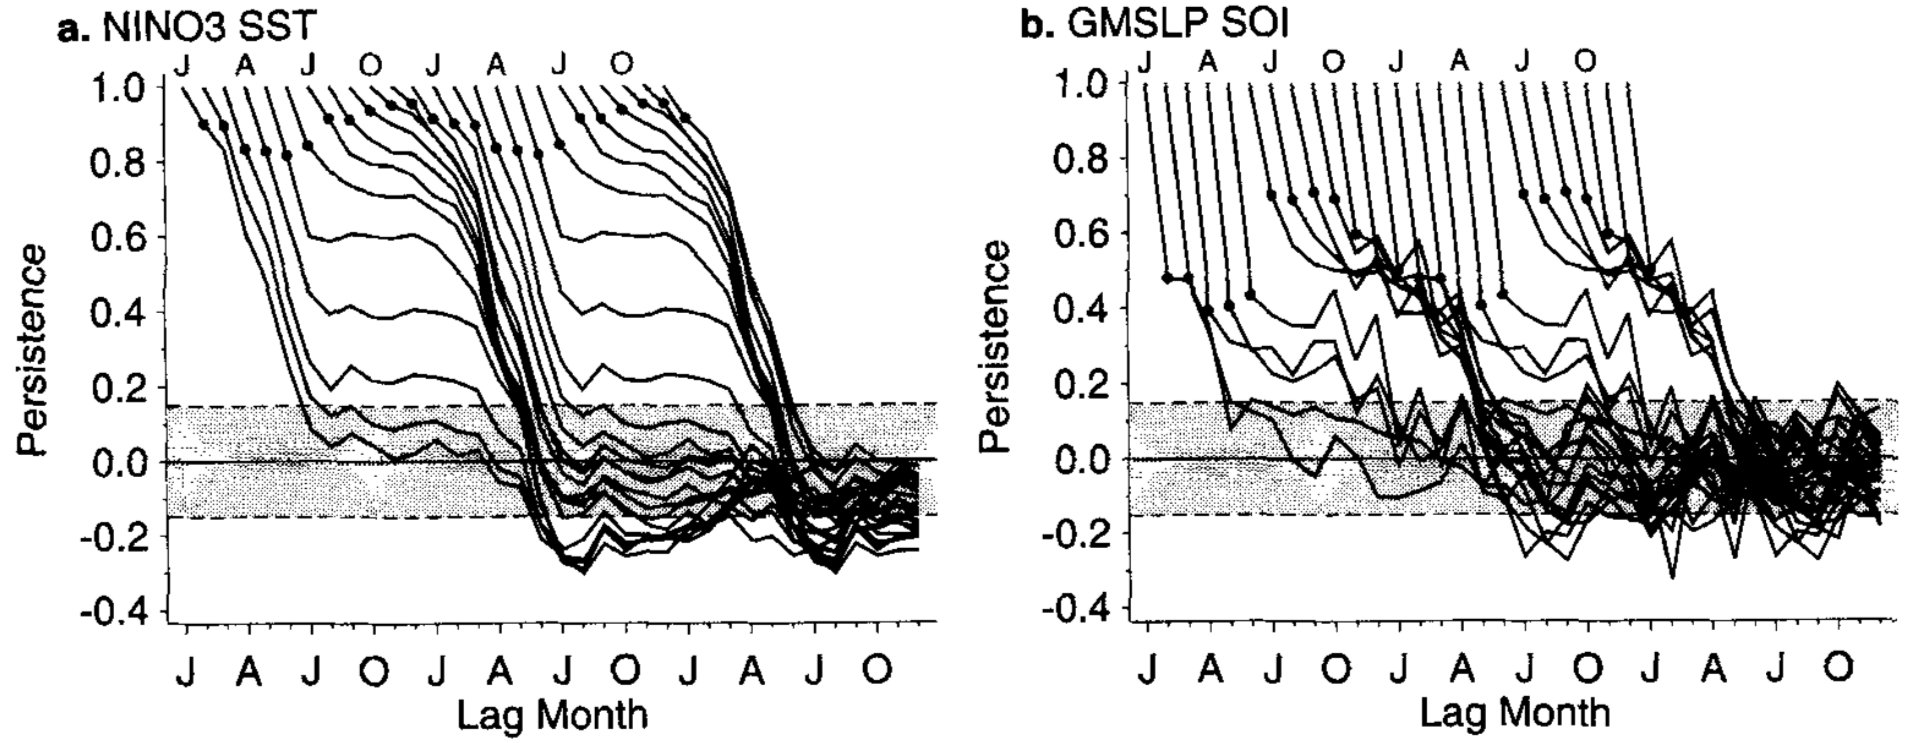
\includegraphics[width=\textwidth]{data/persistence_sst_soi}
\caption[Persistence]{Extracted from \cite{torrence1998annual}: graphs showing the persistence between different months of the year. (a) Persistence of NINO3 surface sea temperature (SST) with each curve shifted to line up with the starting month on the top axis (JAJO=January, April, July, October), and the corresponding lag month on the lower axis. The black dots show the lag-1 persistence, and all twelve curves for one year were repeated for clarity. (b) Features the same analysis but for the Southern Oscillation Index (SOI). }
\label{fig:persistence_sst_soi}
\end{figure}

\section{Origins of the spring predictability barrier}

\section{Overcoming the spring predictability barrier}

\section{Conclusions}

% Creating a sensible and logical narrative is so difficult 

% Identify the topic
% Identify issues with the model
% Identify data and evidence that suggests model needs revising
% Suggest and defend new model or models

\clearpage

%\nocite{wang2017nino}
%\nocite{ruddiman_climate}
\bibliographystyle{agsm}
\bibliography{el_nino}

\end{document}